\section{Open issues and expected achievements}\label{sec:issues}

\begin{figure}[ht]
  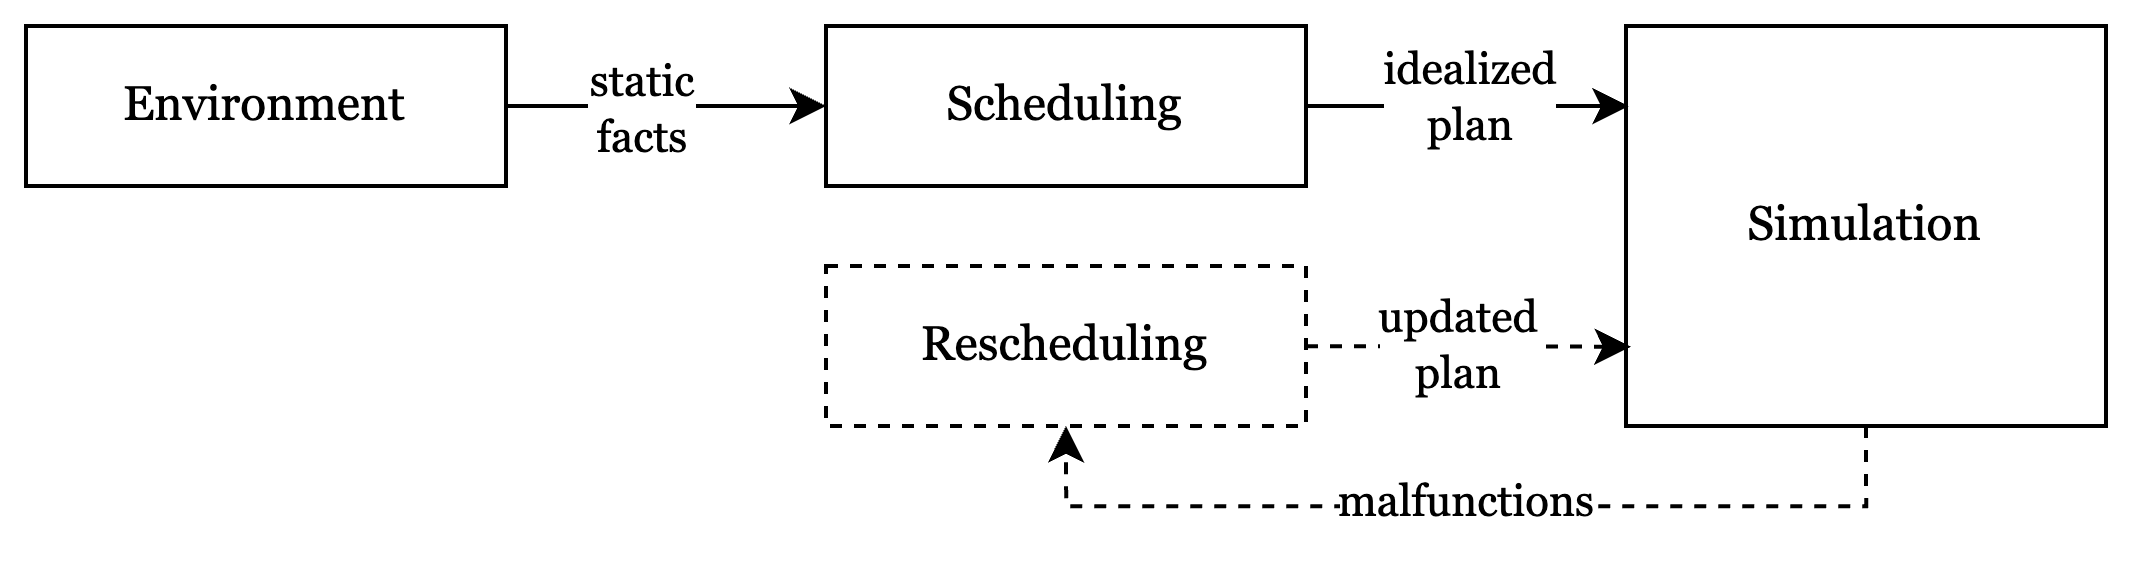
\includegraphics[width=0.8\linewidth, keepaspectratio]{figures/flowchart.png}
  \caption{Logical flow of the \textit{flaspland} system. The dashed lines represent the proposed extension to handle malfunctions}
  \label{fig:flowchart}
\end{figure}

The next significant milestone has to do with handling stochastic malfunctions.
So far, they have been overlooked.
Generally, railway routing and scheduling problems can be viewed in two stages:
\begin{enumerate}
\item \textbf{Planning.} Planning under ideal conditions is known as the vehicle scheduling problem (VSP).
\item \textbf{Execution.} Developing new plans under realistic conditions once execution has already begun is known as the vehicle rescheduling problem (VRSP).
\end{enumerate}
So far, our encodings have been well suited for the VSP,
as we pass along plans in a single-shot solving fashion.
In the future, we will need to adjust our architecture
to function as a two-way channel,
to pass forward calculated train plans,
as well as to report back changes from the simulation to our encodings,
as shown in Figure~\ref{fig:flowchart}.
Concurrently, the encodings will need to shift toward
a multi-shot solving paradigm, to account for changes in current conditions.

In principle, the logic of a VSP encoding could be recycled
by treating a the state of the simulation following a malfunction
as a \textit{fresh start} (i.e. a new environment, as if the current state of the trains were their new starting conditions),
but if conventional wisdom prevails,
benefits exist by retaining information that has already been learned.

Beyond this, my sights are set on tackling the individual problems that comprise railway systems.
We will continue to build a community of those who enroll in our railway scheduling graduate course
and those who choose to write the theses with us on this topic.

%
%%% Local Variables:
%%% mode: LaTeX
%%% TeX-master: "paper"
%%% End:
